\chapter{DataRural}\label{chp:PROPOSTA}

A gestão de dados tornou-se uma dimensão cada vez mais relevante para universidades, sobretudo em instituições que produzem informações acadêmicas, administrativas e experimentais em diferentes setores. Ainda assim, é comum que esses dados permaneçam distribuídos em arquivos locais, planilhas compartilhadas informalmente, sistemas internos pouco integrados ou repositórios que não oferecem documentação suficiente para sua interpretação posterior. Quando isso ocorre, o valor dos dados diminui com o tempo, pois sua reutilização passa a depender do conhecimento individual de quem os produziu ou armazenou.

No contexto da UFRRJ, esse problema pode afetar tanto atividades de pesquisa quanto ações de gestão institucional. Dados de experimentos, levantamentos, projetos de extensão, indicadores acadêmicos ou registros administrativos podem ter utilidade para diferentes públicos, desde que estejam descritos, licenciados e organizados de maneira compreensível. Assim, a simples existência de arquivos digitais não garante transparência, reprodutibilidade ou reaproveitamento científico. É necessário oferecer um ambiente que trate o conjunto de dados como um artefato institucional, com autoria, histórico, permissões e condições claras de uso.

Com base nessa necessidade, este trabalho propõe a Plataforma Institucional de Datasets da UFRRJ, chamada neste projeto de \textit{DataRural}. A proposta consiste em uma aplicação web voltada à publicação, consulta, atualização e organização de datasets institucionais, tendo o formato CSV como ponto de partida. A escolha por esse formato se justifica por sua simplicidade, ampla adoção e compatibilidade com ferramentas de análise de dados, sem impedir que a plataforma evolua futuramente para outros formatos ou para integrações diretas com bases de dados.

O DataRural parte de referências conhecidas no ecossistema de dados, como Kaggle, portais de dados abertos e repositórios científicos. No entanto, seu foco não é reproduzir integralmente nenhuma dessas soluções. A intenção é adaptar conceitos consolidados, como publicação de datasets, hierarquia de usuários e licenciamento, para uma realidade universitária específica. Dessa forma, a plataforma busca apoiar tanto a divulgação pública de dados quanto o trabalho colaborativo de grupos, laboratórios e unidades acadêmicas.

\section{Trabalhos relacionados}

Antes da definição das funcionalidades do DataRural, foram observadas plataformas voltadas ao compartilhamento, à preservação ou à exploração de dados. A análise a seguir combina estudos publicados e observação das interfaces, distinguindo as contribuições da literatura dos elementos visíveis nas capturas de tela. Kaggle, Zenodo e Figshare são discutidos como referências para a concepção do projeto, e não como soluções submetidas a uma avaliação experimental neste trabalho.

\subsection{Kaggle}

O Kaggle reúne datasets, competições e notebooks utilizados em atividades de ciência de dados. Sua dimensão colaborativa é examinada por \citeonline{quaranta2022notebooks}, que analisaram 1.380 notebooks da plataforma em um estudo sobre boas práticas de colaboração. Os autores identificaram diferenças entre o conhecimento das práticas e sua adoção, destacando a importância da documentação e do suporte oferecido pelas ferramentas. Para o DataRural, essa discussão reforça que disponibilizar dados deve ser acompanhado de informações que permitam compreendê-los e reutilizá-los.

A \reffigure{fig:kaggle_interface} apresenta a página inicial do Kaggle\footnote{Disponível em: \url{https://www.kaggle.com/}. Acesso em: 14 set. 2026.}, com acesso à busca, às competições e ao cadastro, além de uma apresentação dos públicos atendidos. Na captura, a plataforma destaca desenvolvedores de inteligência artificial, organizações e pesquisadores. Essa organização visual contextualiza sua orientação comunitária e a articulação entre dados, desafios e atividades de aprendizagem, que serviram de referência para a concepção do DataRural.

\begin{figure}[!htbp]
    \centering
    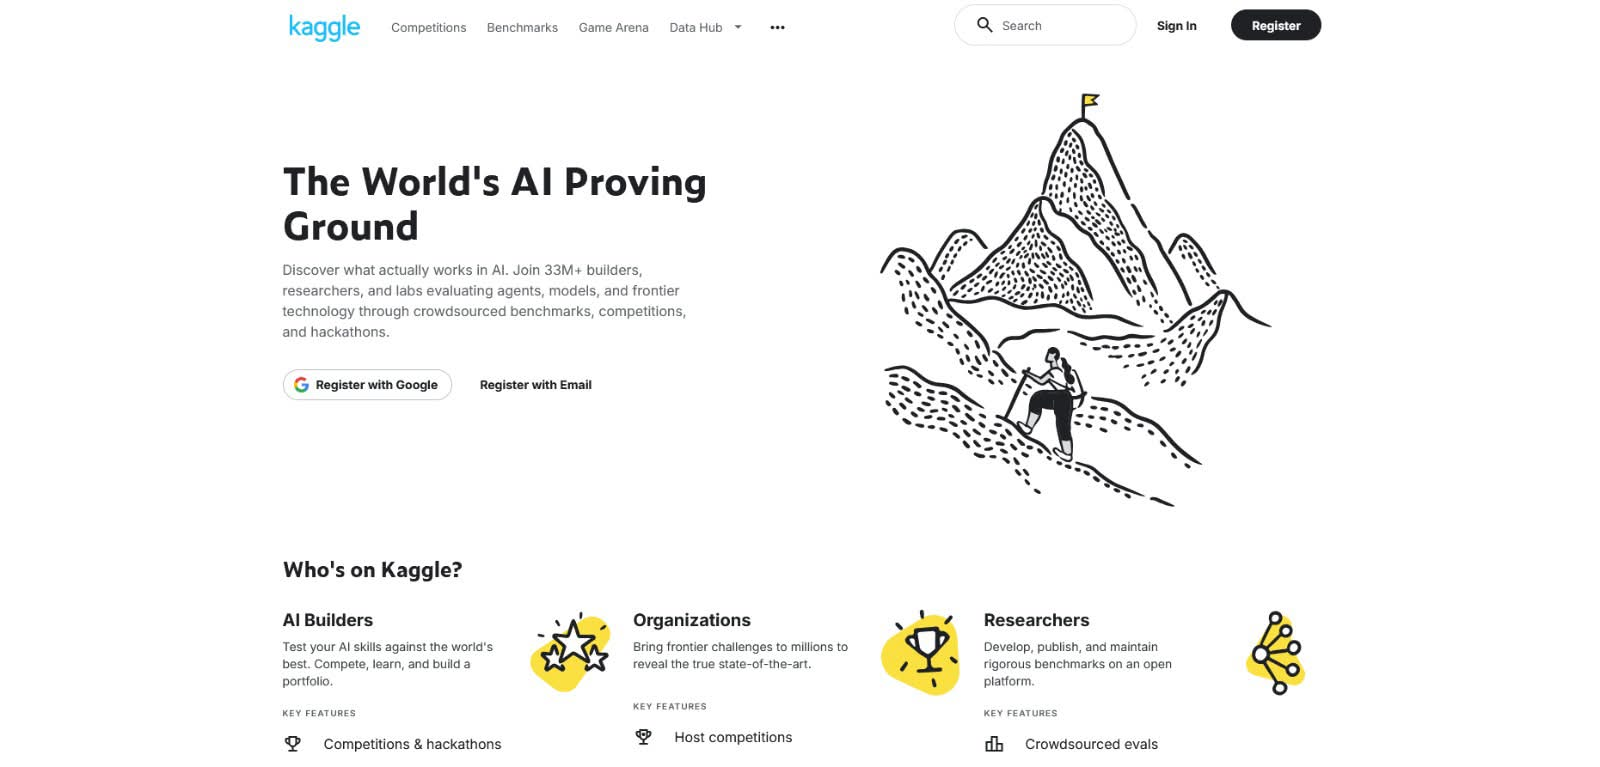
\includegraphics[width=\textwidth,height=0.60\textheight,keepaspectratio]{imagens/kaggle_img.jpg}
    \caption{Página inicial do Kaggle, com navegação para competições, busca e cadastro, além da apresentação dos públicos de desenvolvedores, organizações e pesquisadores.}
    \label{fig:kaggle_interface}
\end{figure}
\FloatBarrier

O aspecto do Kaggle tomado como referência neste trabalho é a articulação entre dados e materiais de análise compartilhados. O DataRural adota um recorte distinto: concentra-se na publicação e na gestão de datasets vinculados à UFRRJ, sem propor competições ou um ambiente de execução de notebooks. A diferença de escopo não implica ausência de colaboração ou de controle de acesso no Kaggle, mas delimita quais conceitos são aproveitados na solução institucional proposta.

\subsection{Zenodo}

O Zenodo é um repositório de propósito geral para divulgação de produtos de pesquisa. \citeonline{conrad2024repositories} o incluem entre as infraestruturas multidisciplinares que apoiam o compartilhamento e a identificação persistente de recursos. Para o DataRural, essa referência destaca a importância de tratar o conjunto de dados como um produto documentado e citável, com autoria e informações que favoreçam sua reutilização.

Além da publicação de artefatos, o Zenodo oferece recursos de organização por comunidades. A \reffigure{fig:zenodo_comunidade} apresenta a tela de gerenciamento de membros da comunidade \textit{Biodiversity Literature Repository}, utilizada como exemplo na documentação oficial da plataforma\footnote{Disponível em: \url{https://help.zenodo.org/docs/communities/manage-members/}. Acesso em: 14 set. 2026.}. A interface reúne busca e filtros, opções de convite e remoção de participantes e a indicação do papel de cada membro. A visibilidade exibida nessa tela diz respeito à participação do membro na comunidade, não à visibilidade de um dataset.

\begin{figure}[!htbp]
    \centering
    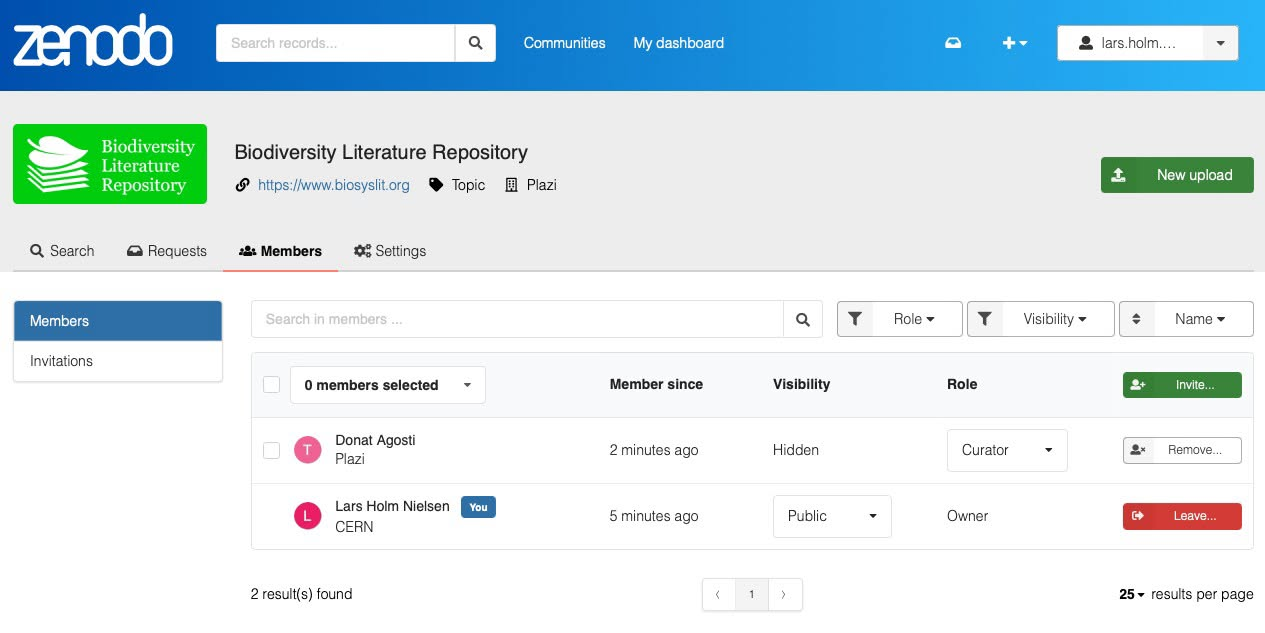
\includegraphics[width=\textwidth,height=0.60\textheight,keepaspectratio]{imagens/zenodo_img.jpg}
    \caption{Gerenciamento de membros de uma comunidade no Zenodo, com identificação dos participantes, papéis, visibilidade da participação e controles de convite e remoção.}
    \label{fig:zenodo_comunidade}
\end{figure}
\FloatBarrier

Esse exemplo evidencia que a colaboração e a diferenciação de responsabilidades também fazem parte do Zenodo. Para o DataRural, a referência contribui para discutir a organização de equipes e o controle das operações sobre conjuntos compartilhados. A proposta deste trabalho não se diferencia pela simples existência de grupos ou papéis, mas pela concepção de uma aplicação própria voltada ao contexto da UFRRJ, na qual os fluxos de publicação, os metadados e as regras de acesso são definidos em função do escopo institucional do projeto.

\subsection{Figshare}

O Figshare também integra o conjunto de repositórios de propósito geral discutido por \citeonline{conrad2024repositories}. O estudo registra seu uso como base tecnológica do repositório 4TU.ResearchData, evidenciando que uma infraestrutura geral pode sustentar serviços voltados a uma comunidade específica. Essa experiência é pertinente ao DataRural por aproximar o compartilhamento de produtos acadêmicos das necessidades de organização institucional.

A \reffigure{fig:figshare_interface} apresenta uma captura da página inicial do Figshare\footnote{Disponível em: \url{https://figshare.com/}. Acesso em: 14 set. 2026.}. Na parte superior, a interface reúne navegação pelo acervo, busca, autenticação e cadastro. A área central destaca o armazenamento, o compartilhamento e a descoberta de resultados de pesquisa, além de indicar soluções destinadas a instituições e editoras. Para a concepção do DataRural, essa apresentação contribui como referência para reunir, na entrada da plataforma, os caminhos de consulta ao acervo e de participação dos usuários.

\begin{figure}[!htbp]
    \centering
    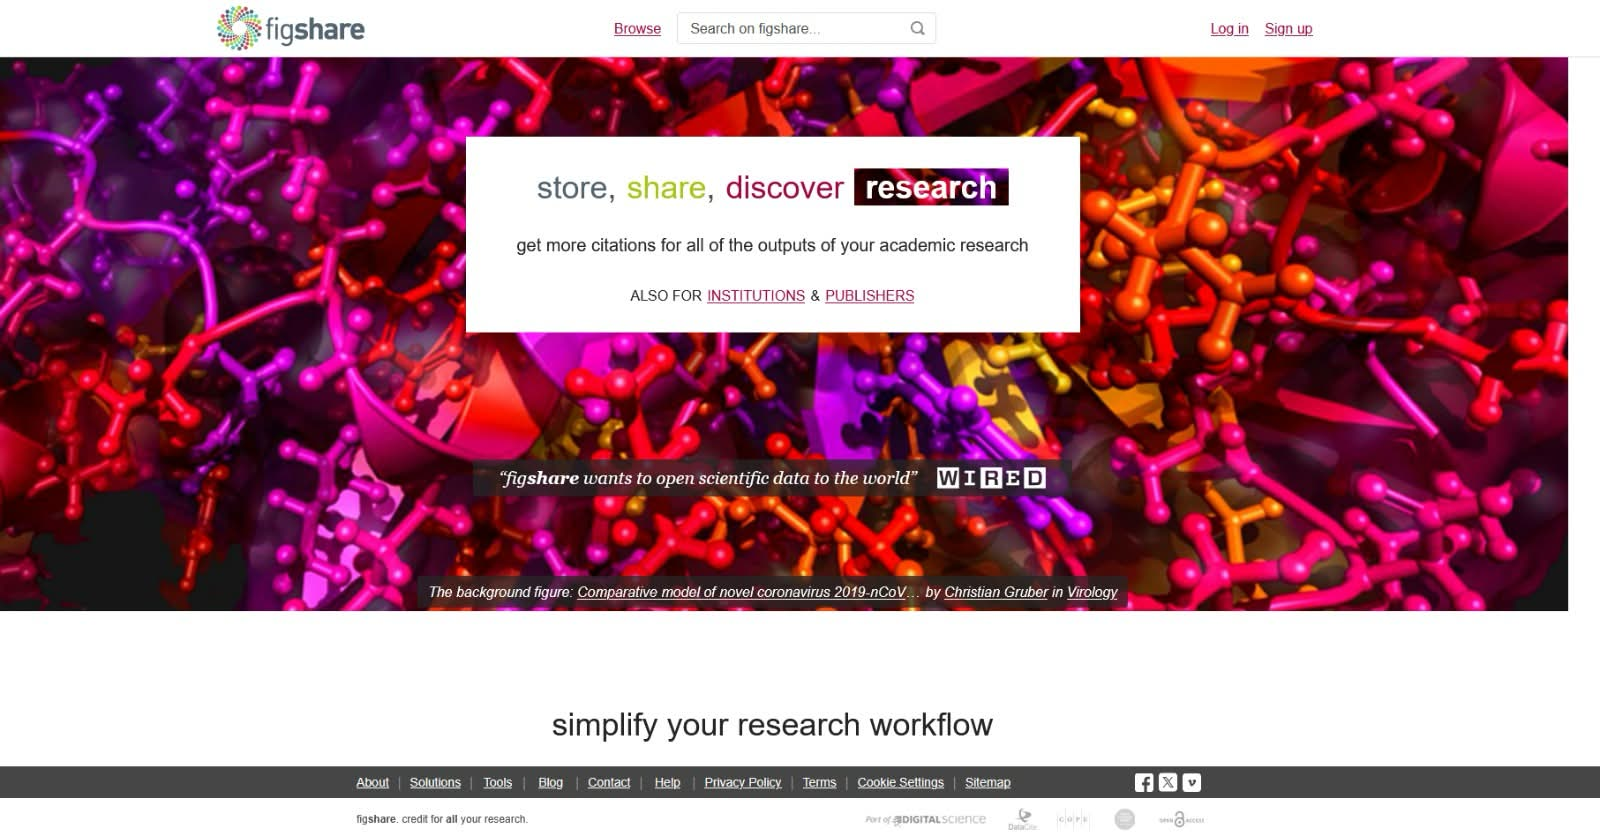
\includegraphics[width=\textwidth,height=0.60\textheight,keepaspectratio]{imagens/figshare_img.jpg}
    \caption{Página inicial do Figshare, com busca e navegação pelo acervo, acesso à conta e destaque para o compartilhamento de resultados de pesquisa e as soluções para instituições e editoras.}
    \label{fig:figshare_interface}
\end{figure}
\FloatBarrier

A indicação de soluções institucionais na própria página reforça que o atendimento a universidades não é uma característica exclusiva do DataRural. A contribuição pretendida neste trabalho está na concepção de uma aplicação própria para a UFRRJ, com metadados, organização de grupos e regras de acesso definidos para o contexto do projeto. Assim, o Figshare serve como referência para a divulgação de produtos acadêmicos, enquanto o DataRural explora a articulação dessas práticas com as necessidades locais de gestão e colaboração.

\section{Visão geral do sistema}

O DataRural é uma aplicação web que centraliza a publicação, consulta e gestão de datasets institucionais. A plataforma foi concebida para atender a dois perfis principais de usuário: o usuário comum, que publica e reutiliza dados, e o administrador, responsável pela manutenção da plataforma, gerenciamento de usuários e configuração de áreas temáticas. Alguns recursos, como a consulta e o download de datasets públicos, estão disponíveis mesmo para usuários não autenticados, ampliando o alcance da informação.

A unidade central do sistema é o dataset. Cada conjunto de dados é descrito por metadados como título, descrição, área temática, unidade responsável, região, período, palavras-chave e licença. Essas informações fornecem o contexto necessário para sua compreensão e reutilização. A visibilidade controla o acesso: datasets públicos são acessíveis a qualquer visitante, enquanto datasets privados ficam restritos ao proprietário ou ao grupo ao qual estão vinculados.

O sistema adota o versionamento como princípio estrutural. Cada atualização de um conjunto de dados gera uma nova versão, preservando o histórico completo de modificações e permitindo rastrear qual versão foi utilizada em determinada análise ou relatório. Versões podem ser excluídas de forma lógica e restauradas quando necessário.

Os grupos colaborativos constituem outro elemento central da plataforma. Eles representam laboratórios, equipes ou unidades institucionais e permitem que múltiplos usuários trabalhem de forma coordenada sobre os mesmos datasets, com papéis bem definidos: dono, administrador, editor e leitor. Essa estrutura de colaboração diferencia o DataRural de repositórios de uso individual, tornando-o adequado tanto para a divulgação pública de dados quanto para o trabalho interno de equipes acadêmicas.

\section{Concepção da interface e prototipação}\label{sec:prototipacao}

A evolução da interface do DataRural é apresentada a partir de dois registros distintos: a primeira interface do projeto, centrada no envio de arquivos CSV, e um \textit{mockup} elaborado com auxílio do Claude para explorar a organização das informações e os caminhos de navegação. A primeira registra uma versão inicial do sistema; o segundo representa uma proposta visual, cujos elementos não correspondem necessariamente às funcionalidades implementadas. Essa distinção permite contextualizar as escolhas de interface e sua relação com a solução descrita no Capítulo~\ref{chp:EXPERIMENTOS}.

\subsection{Primeira interface do projeto}

A \reffigure{fig:interface_inicial} apresenta a primeira interface do DataRural, com um formulário de envio de conjuntos de dados. A tela reúne campos para o nome do dataset, a versão, a seleção de um arquivo CSV e observações destinadas ao \texttt{README.md}, além de um botão de acesso ao visualizador. A identidade visual ainda mantém a identificação do \textit{Starter Kit} do AdonisJS, diferentemente das telas da plataforma apresentadas no capítulo de implementação.

\begin{figure}[!htbp]
    \centering
    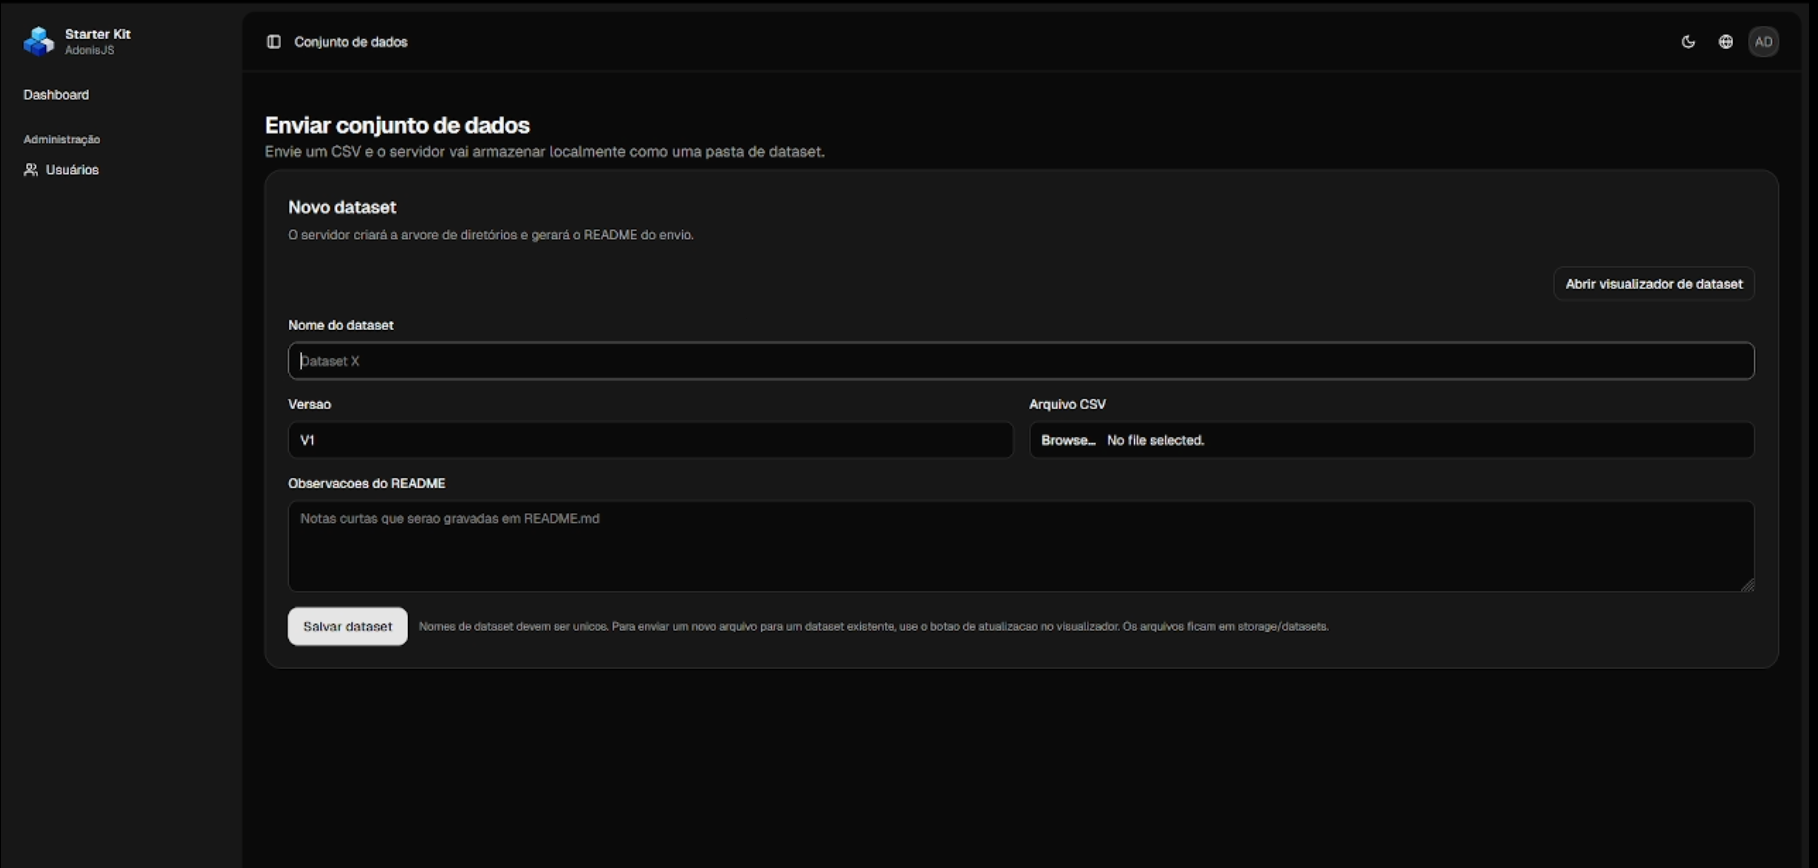
\includegraphics[width=\textwidth,height=0.60\textheight,keepaspectratio]{imagens/interface-inicial.png}
    \caption{Primeira interface do DataRural, com formulário de envio de CSV, identificação do dataset, versão e observações para o README.}
    \label{fig:interface_inicial}
\end{figure}
\FloatBarrier

Nesse registro, o envio do arquivo e sua identificação estão concentrados em um único formulário, e a documentação aparece como um campo de observações livres. Na versão apresentada na Seção~\ref{sec:impl_publicacao}, a publicação é organizada em cinco etapas, com espaços específicos para metadados, dicionário de dados, licença e visibilidade. O contraste documenta a ampliação das informações solicitadas e a mudança na organização do fluxo, sem constituir, por si só, evidência de melhoria de usabilidade.

A concepção da interface também incluiu a exploração da experiência de consulta aos conjuntos publicados. O mockup discutido a seguir aborda essa dimensão: em vez de representar outra versão do formulário de envio, apresenta uma proposta para a página de detalhes de um dataset, destacando sua documentação e as informações necessárias à reutilização.

\subsection{Geração e revisão do protótipo}

O mockup foi gerado com auxílio do Claude a partir do minimundo do projeto, entendido como a descrição do contexto institucional, dos usuários, das entidades e das regras que delimitam o sistema. Esse contexto reúne as necessidades de publicação de arquivos CSV, descrição dos conjuntos, consulta pública, colaboração por grupos e preservação do histórico. Sua utilização como entrada para a geração visual buscou aproximar a proposta de interface das necessidades do DataRural, e não apenas produzir uma composição gráfica genérica.

A geração foi acompanhada pela participação dos autores na análise da proposta e no fornecimento de feedback para seu refinamento. Essa participação caracteriza a revisão humana no processo, também denominada \textit{human in the loop}: a ferramenta auxilia na elaboração visual, enquanto a avaliação da adequação ao minimundo e as decisões sobre o que incorporar ao projeto permanecem sob responsabilidade dos autores. Trata-se de uma atividade de concepção, e não de uma avaliação de usabilidade com usuários da universidade.

A \reffigure{fig:mockup_dataset} apresenta um recorte do protótipo da página de detalhes de um dataset. A imagem registra uma proposta de organização da interface, não uma captura do sistema em funcionamento. Os nomes, valores, gráficos e contagens exibidos têm função ilustrativa e não representam resultados de testes nem indicadores de utilização do DataRural.

\begin{figure}[!htbp]
    \centering
    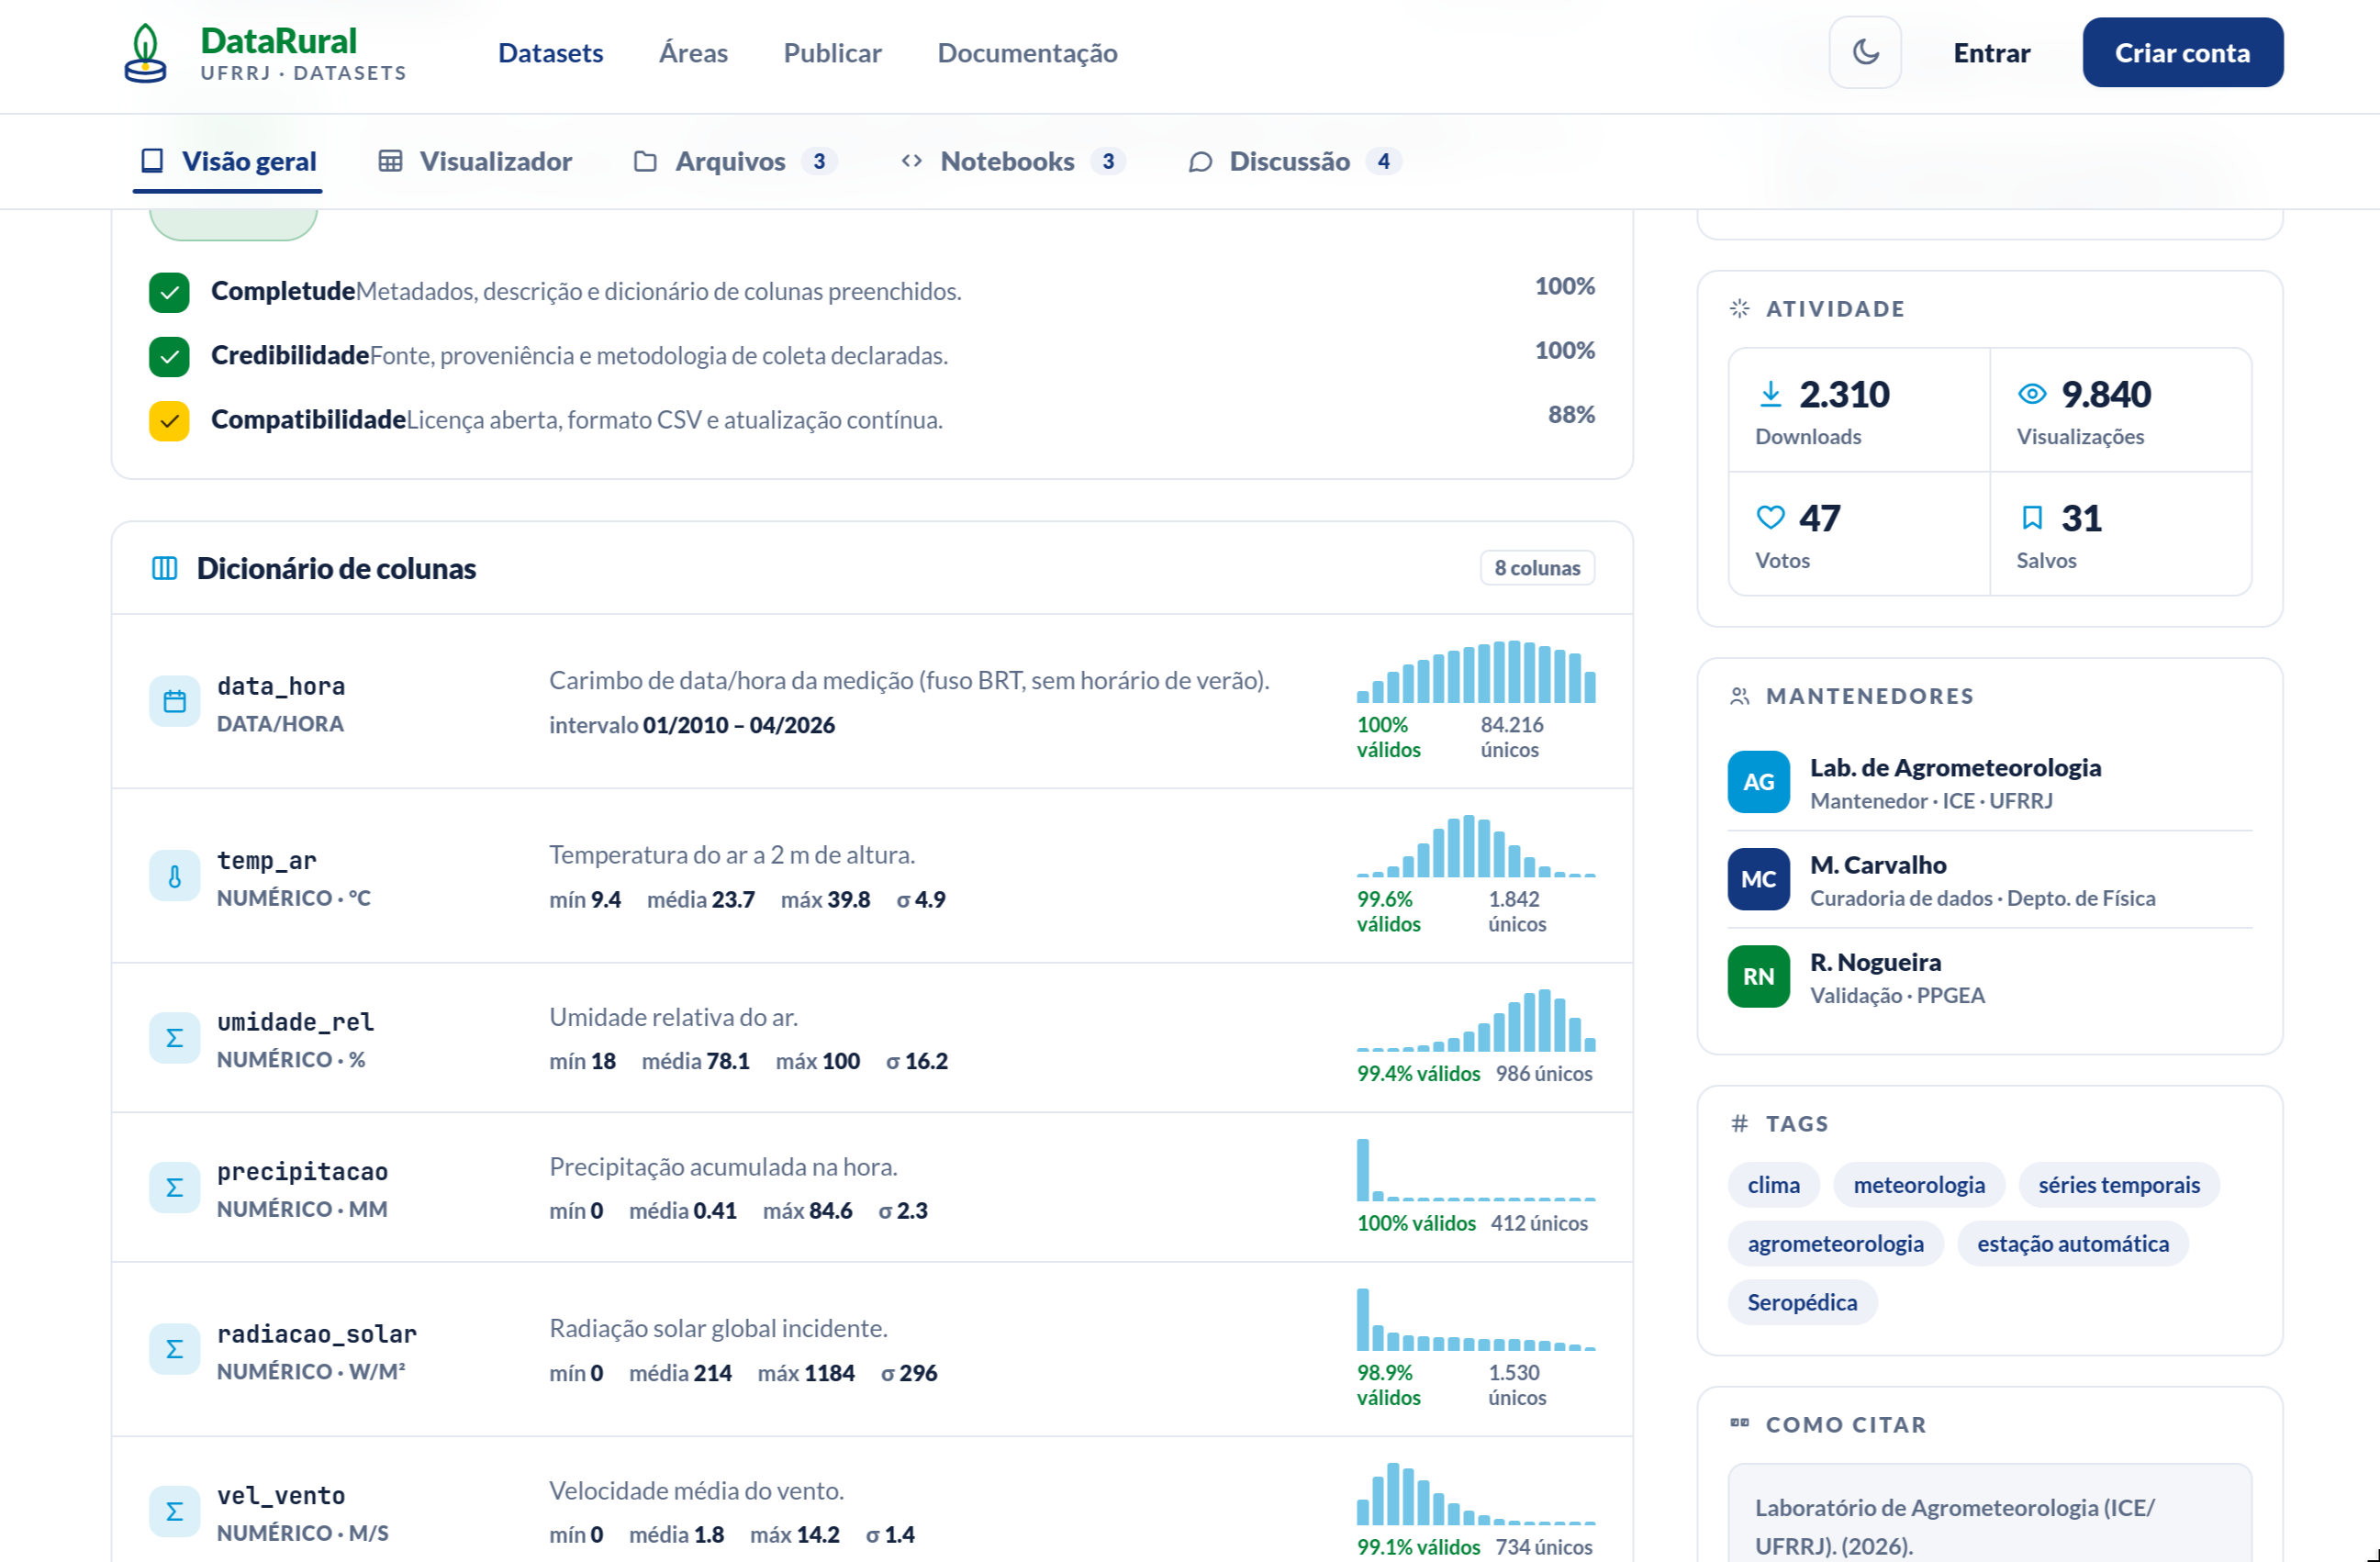
\includegraphics[width=\textwidth,height=0.68\textheight,keepaspectratio]{imagens/claude-design.png}
    \caption{Recorte do mockup da página de detalhes de um dataset do DataRural, com dicionário de colunas, indicadores e informações dos responsáveis. Os dados exibidos são ilustrativos.}
    \label{fig:mockup_dataset}
\end{figure}
\FloatBarrier

\subsection{Discussão da proposta visual}

No protótipo, o dicionário de colunas ocupa a região central, associando nomes de variáveis a descrições, tipos, unidades de medida e representações resumidas dos valores. Essa disposição dá destaque à interpretação dos dados: antes de obter o arquivo, o visitante deve encontrar informações que o ajudem a reconhecer o conteúdo e a avaliar sua adequação ao uso pretendido. A composição visual expressa, portanto, a preocupação com a documentação por atributo, complementar aos metadados gerais do conjunto.

A coluna lateral agrupa informações sobre mantenedores, palavras-chave, atividade e citação. A presença desses elementos permite discutir diferentes dimensões da publicação: a identificação dos responsáveis, a localização por tema, as formas de referência ao conjunto e o acompanhamento das interações. Já a organização em abas separa a visão geral de áreas destinadas à visualização e aos arquivos. Esses elementos funcionam como referências para a organização da experiência de consulta, sem que sua presença no mockup comprove a implementação dos mecanismos correspondentes.

O protótipo também apresenta abas de \textit{notebooks} e discussão, que não são apresentadas como funcionalidades implementadas neste trabalho. A distinção evidencia que a exploração visual contemplou possibilidades mais amplas do que a entrega descrita no Capítulo~\ref{chp:EXPERIMENTOS}. A solução desenvolvida prioriza publicação e consulta de CSV, metadados, controle de acesso, grupos e histórico de versões. Na página de detalhes implementada, apresentada na Seção~\ref{sec:impl_exploracao}, a navegação reúne visão geral, visualizador, arquivos e versões. Assim, o mockup é tratado como apoio à concepção, e não como uma especificação de que todos os elementos ilustrados seriam entregues nesta etapa.

\subsection{Fluxos de uso previstos}\label{sec:fluxos_propostos}

A proposta organiza o uso da plataforma em três fluxos complementares: descoberta de dados, publicação e manutenção do acervo. Essa organização relaciona as necessidades dos usuários aos requisitos apresentados na seção seguinte, sem vincular sua descrição a uma tela específica.

No fluxo de descoberta, o visitante deve poder localizar datasets públicos, consultar seus metadados e obter os arquivos de interesse. A busca e a classificação por área temática devem facilitar a seleção dos conjuntos, enquanto a apresentação da licença e de uma prévia tabular deve apoiar a avaliação inicial do material antes de sua reutilização.

O fluxo de publicação deve reunir o envio dos arquivos, a descrição do conjunto e a definição das condições de uso e de acesso. A identificação do responsável permite associar a publicação a um usuário e, quando necessário, a um grupo. A manutenção do acervo deve permitir atualizar os dados sem perder suas versões anteriores, além de controlar alterações de visibilidade e operações de exclusão conforme as permissões atribuídas.

Esses fluxos orientam a concepção da plataforma. As interfaces do sistema desenvolvido e os mecanismos utilizados para realizá-los são apresentados na Seção~\ref{sec:fluxos} do Capítulo~\ref{chp:EXPERIMENTOS}, distinguindo a definição da proposta da apresentação de sua implementação.

\section{Requisitos do sistema}

Os requisitos apresentados nesta seção organizam as capacidades esperadas para a plataforma. Eles foram definidos a partir dos objetivos do projeto e procuram traduzir, em funcionalidades e restrições, a proposta de uma solução institucional para publicação e gestão de datasets. Para facilitar a leitura, os requisitos foram separados em funcionais, não funcionais e regras de negócio.

\subsection{Requisitos funcionais}

A Tabela~\ref{tab:requisitos_funcionais} apresenta os requisitos funcionais definidos para o DataRural. Esses requisitos descrevem as operações que a plataforma deve disponibilizar aos seus usuários, incluindo publicação, consulta, versionamento, colaboração e administração.

\begin{longtable}{p{0.15\textwidth}p{0.75\textwidth}}
\caption{Requisitos funcionais do DataRural: operações previstas para publicação, consulta e gestão de datasets, colaboração entre usuários e administração da plataforma.}\label{tab:requisitos_funcionais}\\
\toprule
\textbf{Código} & \textbf{Descrição} \\
\midrule
\endfirsthead
\toprule
\textbf{Código} & \textbf{Descrição} \\
\midrule
\endhead
RF-01 & Permitir o upload de \textit{datasets} em formato CSV. \\
RF-02 & Permitir o upload de múltiplos arquivos CSV por versão do dataset. \\
RF-03 & Permitir a criação de grupos de usuários com papéis (dono, admin, editor, visualizador). \\
RF-04 & Permitir a criação de \textit{datasets} privados. \\
RF-05 & Permitir alternar a visibilidade (público/privado) de um dataset. \\
RF-06 & Permitir o versionamento de \textit{datasets}. \\
RF-07 & Permitir a restauração de versões anteriores de um dataset. \\
RF-08 & Permitir a exclusão lógica (\textit{soft delete}) de versões. \\
RF-09 & Permitir a descrição e o licenciamento de \textit{datasets} publicados. \\
RF-10 & Permitir a classificação de datasets por metadados (área, unidade, período, região, tags). \\
RF-11 & Permitir o download individual de arquivos de um dataset. \\
RF-12 & Permitir o download de todos os arquivos de uma versão em formato ZIP. \\
RF-13 & Permitir o registro e autenticação de usuários. \\
RF-14 & Permitir a edição de perfil do usuário (nome, bio, avatar, instituição, localização). \\
RF-15 & Permitir que usuários curtam datasets. \\
RF-16 & Permitir que usuários favoritem datasets para acesso rápido. \\
RF-17 & Permitir a exploração e busca de datasets com filtro por área temática. \\
RF-18 & Exibir uma prévia das primeiras linhas dos arquivos CSV de um dataset. \\
RF-19 & Permitir a atribuição de datasets a grupos. \\
RF-20 & Permitir a exclusão de datasets apenas pelo proprietário ou membro autorizado do grupo. \\
RF-21 & Oferecer um painel administrativo para gestão de usuários e áreas temáticas. \\
RF-22 & Registrar trilha de auditoria para alterações nas entidades principais. \\
RF-23 & Oferecer suporte a internacionalização (i18n). \\
RF-24 & Exibir perfis públicos de usuários. \\
\bottomrule
\end{longtable}

\subsection{Requisitos não funcionais}

Os requisitos não funcionais, apresentados na Tabela~\ref{tab:requisitos_nao_funcionais}, estabelecem restrições e qualidades esperadas para a plataforma. Eles orientam decisões de implementação relacionadas a segurança, organização do código, preservação do histórico e compatibilidade.

\begin{longtable}{p{0.15\textwidth}p{0.75\textwidth}}
\caption{Requisitos não funcionais do DataRural: critérios de segurança, compatibilidade, clareza da interface, rastreabilidade e organização do software.}\label{tab:requisitos_nao_funcionais}\\
\toprule
\textbf{Código} & \textbf{Descrição} \\
\midrule
\endfirsthead
\toprule
\textbf{Código} & \textbf{Descrição} \\
\midrule
\endhead
RNF-01 & A solução deve ser disponibilizada como aplicação web responsiva e compatível com navegadores atuais. \\
RNF-02 & As senhas devem ser armazenadas por meio de representação criptográfica segura. \\
RNF-03 & O acesso a rotas protegidas deve ser controlado por \textit{middleware} de autenticação. \\
RNF-04 & Os arquivos enviados devem ser validados, considerando inicialmente apenas o formato CSV. \\
RNF-05 & O código deve manter separação entre interface, regras de negócio, persistência e armazenamento de arquivos. \\
RNF-06 & A estrutura da plataforma deve permitir evolução para novos formatos e novas fontes de dados. \\
RNF-07 & O histórico de versões deve ser preservado para manter rastreabilidade das alterações. \\
RNF-08 & A interface deve apresentar metadados, permissões e licenças de forma clara ao usuário. \\
RNF-09 & As principais entidades devem ser auditáveis. \\
RNF-10 & A organização modular do sistema deve favorecer manutenção e expansão gradual. \\
\bottomrule
\end{longtable}

\subsection{Regras de negócio}

As regras de negócio, listadas na Tabela~\ref{tab:regras_negocio}, definem condições que devem ser respeitadas pela plataforma independentemente da tecnologia adotada. Elas delimitam permissões, restrições de formato e políticas de visibilidade que orientam o comportamento esperado do sistema.

\begin{longtable}{p{0.15\textwidth}p{0.75\textwidth}}
\caption{Regras de negócio do DataRural: condições de publicação, licenciamento e acesso aos datasets e restrições que orientam o funcionamento da plataforma.}\label{tab:regras_negocio}\\
\toprule
\textbf{Código} & \textbf{Descrição} \\
\midrule
\endfirsthead
\toprule
\textbf{Código} & \textbf{Descrição} \\
\midrule
\endhead
RN-01 & A publicação de \textit{datasets} é restrita a usuários autenticados. \\
RN-02 & Usuários não registrados podem visualizar e fazer download de \textit{datasets} públicos. \\
RN-03 & Todo \textit{dataset} publicado deve possuir uma licença associada. \\
RN-04 & \textit{Datasets} não publicados são visíveis apenas pelo usuário proprietário ou membros do grupo associado. \\
RN-05 & Nomes de \textit{datasets} devem ser únicos no sistema. \\
RN-06 & Cada arquivo CSV enviado deve ter no máximo 25 MB. \\
RN-07 & Membros de grupo com papel de dono, admin ou editor podem editar datasets do grupo. \\
RN-08 & Apenas membros com papel de dono ou admin podem excluir versões de um dataset do grupo. \\
RN-09 & A exclusão de versões é lógica (\textit{soft delete}), preservando os dados no sistema. \\
\bottomrule
\end{longtable}

\section{Controle de acesso}\label{sec:controle_acesso}

A plataforma armazena tanto dados públicos quanto dados privados, o que exige a identificação dos usuários e a restrição de operações de acordo com suas responsabilidades. A autenticação verifica o controle dos autenticadores associados à conta, conforme a abordagem das diretrizes de identidade digital do NIST \cite{nist2025passwords}. A autorização determina quais recursos e operações são permitidos e pode ser organizada por papéis, conforme o modelo de \citeonline{sandhu2000rbac}.

No DataRural, a autenticação ocorre quando o usuário apresenta suas credenciais. Após a verificação, o servidor mantém a identidade autenticada entre diferentes requisições por meio de uma sessão \cite{nist2025passwords}. Um identificador de sessão é enviado ao navegador e utilizado nas interações seguintes, permitindo que o servidor reconheça o usuário sem solicitar novamente a senha em cada página. As senhas não são armazenadas em texto simples: utiliza-se uma função de derivação acompanhada de um valor aleatório (\textit{salt}), conforme recomendado pelo NIST \cite{nist2025passwords}.

A autorização é organizada por meio do controle de acesso baseado em papéis, conhecido como RBAC (\textit{role-based access control}) \cite{sandhu2000rbac}. Nesse modelo, permissões são associadas a papéis, e cada usuário recebe um ou mais desses papéis. O acesso é decidido a partir das funções atribuídas, evitando que cada permissão precise ser configurada individualmente para cada pessoa.

No DataRural, os papéis operam em dois níveis. Os papéis globais distinguem usuários comuns de administradores da plataforma, sendo registrados na entidade \textit{roles} e associados ao campo \textit{role\_id} do usuário. Os papéis contextuais são válidos apenas dentro de um grupo e definem o que cada membro pode fazer em relação aos datasets daquele grupo. Assim, a mesma pessoa pode administrar uma equipe e atuar apenas como leitora em outra.

A verificação de acesso é aplicada pelo servidor antes que a requisição alcance a operação principal, por meio de componentes de \textit{middleware}. Um \textit{middleware} de autenticação impede o acesso de visitantes a rotas protegidas, enquanto a autorização mais específica também considera o recurso solicitado, pois estar autenticado não significa possuir permissão para alterar qualquer registro. A interface pode ocultar ou desabilitar ações não permitidas para tornar o sistema mais compreensível, mas essa medida não substitui a validação no servidor, pois requisições podem ser construídas sem utilizar os botões da página.

\section{Modelagem de dados}

A modelagem de dados do DataRural foi orientada pelas responsabilidades identificadas ao longo da proposta. O dataset ocupa a posição central do modelo, enquanto as demais entidades oferecem suporte a autenticação, autoria, licenciamento, versionamento e colaboração. A estrutura permite que a plataforma trate o arquivo enviado e suas informações descritivas como partes de um mesmo registro institucional.

A adoção de um banco de dados relacional se mostra adequada porque as relações do domínio são bem definidas. Usuários publicam datasets, datasets possuem versões, licenças são associadas a datasets e grupos reúnem usuários. Além disso, o modelo facilita a aplicação de restrições de integridade e a consulta estruturada das informações utilizadas pela plataforma.

As subseções a seguir apresentam cada entidade, suas colunas e seus papéis no sistema. A entidade \textit{users} concentra os dados de autenticação e perfil. As entidades \textit{roles} e \textit{groups}/\textit{group\_members} organizam os dois níveis de permissão descritos na seção anterior. A entidade \textit{datasets} reúne os metadados do conjunto publicado, enquanto \textit{dataset\_versions} e \textit{dataset\_version\_files} implementam o mecanismo de versionamento discutido no Capítulo~\ref{chp:FUNDAMENTACAO}. A separação entre o dataset e suas versões merece atenção especial: em vez de tratar cada publicação como um arquivo substituível, o modelo preserva cada estado anterior como uma versão distinta, vinculada ao mesmo registro. Essa decisão foi motivada pela necessidade de rastreabilidade, um dos princípios centrais da gestão de dados de pesquisa, e pela possibilidade de restaurar versões excluídas logicamente, evitando perdas acidentais. Por fim, as entidades \textit{dataset\_likes} e \textit{dataset\_favorites} registram, respectivamente, as curtidas e os favoritos dos usuários, representando formas distintas de interação: a curtida funciona como uma valorização pública, enquanto o favorito cria uma coleção pessoal para acesso rápido. A entidade \textit{audits} registra alterações para fins de rastreabilidade interna.

\subsection{Entidade \textit{users}}

A entidade \textit{users} concentra os dados dos usuários cadastrados. Ela participa dos fluxos de autenticação, autoria, administração e associação com grupos. A Tabela~\ref{tab:entity_users} apresenta suas colunas.

\begin{longtable}{p{0.25\textwidth}p{0.18\textwidth}p{0.47\textwidth}}
\caption{Estrutura da entidade \textit{users} do DataRural, que armazena os dados de autenticação e perfil dos usuários e sua associação a um papel global.}\label{tab:entity_users}\\
\toprule
\textbf{Coluna} & \textbf{Tipo} & \textbf{Descrição} \\
\midrule
\endfirsthead
\toprule
\textbf{Coluna} & \textbf{Tipo} & \textbf{Descrição} \\
\midrule
\endhead
id & Integer & Chave primária do usuário. \\
email & Varchar & E-mail utilizado para identificação e acesso. \\
password & Varchar & Senha armazenada em formato protegido. \\
full\_name & Varchar & Nome completo exibido na plataforma. \\
username & Varchar & Nome de usuário único para identificação na plataforma. \\
bio & Text & Biografia do usuário. \\
avatar & JSON & Metadados do avatar enviado (attachment). \\
avatar\_url & Varchar & URL do avatar externo (login social). \\
institution & Varchar & Instituição à qual o usuário pertence. \\
location & Varchar & Localização do usuário. \\
role\_id & Integer & Papel global atribuído ao usuário. \\
created\_at & Timestamp & Data de criação do registro. \\
updated\_at & Timestamp & Data da alteração mais recente. \\
\bottomrule
\end{longtable}

\subsection{Entidade \textit{roles}}

A entidade \textit{roles} define os papéis globais disponíveis na aplicação, distinguindo usuários comuns de administradores. A Tabela~\ref{tab:entity_roles} apresenta sua estrutura.

\begin{longtable}{p{0.25\textwidth}p{0.18\textwidth}p{0.47\textwidth}}
\caption{Estrutura da entidade \textit{roles} do DataRural, que define os papéis globais de acesso, distinguindo usuários comuns de administradores da plataforma.}\label{tab:entity_roles}\\
\toprule
\textbf{Coluna} & \textbf{Tipo} & \textbf{Descrição} \\
\midrule
\endfirsthead
\toprule
\textbf{Coluna} & \textbf{Tipo} & \textbf{Descrição} \\
\midrule
\endhead
id & Integer & Chave primária do papel. \\
name & Varchar & Nome atribuído ao papel. \\
description & Text & Explicação das permissões associadas. \\
created\_at & Timestamp & Data de criação do registro. \\
updated\_at & Timestamp & Data da alteração mais recente. \\
\bottomrule
\end{longtable}

\subsection{Entidade \textit{groups}}

A entidade \textit{groups} representa espaços colaborativos vinculados a equipes, laboratórios, projetos ou unidades institucionais. A Tabela~\ref{tab:entity_groups} apresenta suas colunas.

\begin{longtable}{p{0.25\textwidth}p{0.18\textwidth}p{0.47\textwidth}}
\caption{Estrutura da entidade \textit{groups} do DataRural, que registra os grupos colaborativos, suas finalidades e os usuários responsáveis por eles.}\label{tab:entity_groups}\\
\toprule
\textbf{Coluna} & \textbf{Tipo} & \textbf{Descrição} \\
\midrule
\endfirsthead
\toprule
\textbf{Coluna} & \textbf{Tipo} & \textbf{Descrição} \\
\midrule
\endhead
id & Integer & Chave primária do grupo. \\
name & Varchar & Nome do grupo colaborativo. \\
description & Text & Descrição da finalidade do grupo. \\
owner\_id & Integer & Usuário responsável pelo grupo. \\
created\_at & Timestamp & Data de criação do registro. \\
updated\_at & Timestamp & Data da alteração mais recente. \\
\bottomrule
\end{longtable}

\subsection{Entidade \textit{group\_members}}

A entidade \textit{group\_members} registra a participação de usuários em grupos e informa o papel exercido por cada membro naquele contexto. A Tabela~\ref{tab:entity_group_members} apresenta sua estrutura.

\begin{longtable}{p{0.25\textwidth}p{0.18\textwidth}p{0.47\textwidth}}
\caption{Estrutura da entidade \textit{group\_members} do DataRural, que associa usuários a grupos colaborativos e registra o papel de cada membro no respectivo grupo.}\label{tab:entity_group_members}\\
\toprule
\textbf{Coluna} & \textbf{Tipo} & \textbf{Descrição} \\
\midrule
\endfirsthead
\toprule
\textbf{Coluna} & \textbf{Tipo} & \textbf{Descrição} \\
\midrule
\endhead
id & Integer & Chave primária da associação. \\
group\_id & Integer & Grupo ao qual o usuário pertence. \\
user\_id & Integer & Usuário associado ao grupo. \\
role & Varchar & Papel exercido no grupo (owner, admin, editor). \\
created\_at & Timestamp & Data de entrada no grupo. \\
updated\_at & Timestamp & Data da alteração mais recente. \\
\bottomrule
\end{longtable}

\subsection{Entidade \textit{licenses}}

A entidade \textit{licenses} mantém as licenças que podem ser vinculadas aos datasets, tornando explícitas as condições de uso e redistribuição. A Tabela~\ref{tab:entity_licenses} apresenta suas colunas.

\begin{longtable}{p{0.25\textwidth}p{0.18\textwidth}p{0.47\textwidth}}
\caption{Estrutura da entidade \textit{licenses} do DataRural, que registra as licenças associáveis aos datasets e suas condições de uso e redistribuição.}\label{tab:entity_licenses}\\
\toprule
\textbf{Coluna} & \textbf{Tipo} & \textbf{Descrição} \\
\midrule
\endfirsthead
\toprule
\textbf{Coluna} & \textbf{Tipo} & \textbf{Descrição} \\
\midrule
\endhead
id & Integer & Chave primária da licença. \\
name & Varchar & Nome resumido da licença. \\
description & Text & Termos ou explicação da licença. \\
created\_at & Timestamp & Data de criação do registro. \\
updated\_at & Timestamp & Data da alteração mais recente. \\
\bottomrule
\end{longtable}

\subsection{Entidade \textit{dataset\_areas}}

A entidade \textit{dataset\_areas} armazena as áreas temáticas disponíveis para classificação dos datasets, permitindo filtragem e navegação por categoria. A Tabela~\ref{tab:entity_dataset_areas} apresenta sua estrutura.

\begin{longtable}{p{0.25\textwidth}p{0.18\textwidth}p{0.47\textwidth}}
\caption{Estrutura da entidade \textit{dataset\_areas} do DataRural, que registra as áreas temáticas utilizadas na classificação dos conjuntos de dados.}\label{tab:entity_dataset_areas}\\
\toprule
\textbf{Coluna} & \textbf{Tipo} & \textbf{Descrição} \\
\midrule
\endfirsthead
\toprule
\textbf{Coluna} & \textbf{Tipo} & \textbf{Descrição} \\
\midrule
\endhead
id & Integer & Chave primária da área. \\
name & Varchar & Nome da área temática. \\
code & Varchar & Código identificador da área. \\
description & Text & Descrição da área. \\
icon & Varchar & Ícone representativo da área. \\
color & Varchar & Cor associada à área. \\
created\_at & Timestamp & Data de criação do registro. \\
updated\_at & Timestamp & Data da alteração mais recente. \\
\bottomrule
\end{longtable}

\subsection{Entidade \textit{datasets}}

A entidade \textit{datasets} reúne os metadados e configurações centrais de cada conjunto de dados publicado. Por meio dela são definidos autoria, licença, visibilidade, status, área, unidade responsável e demais informações necessárias para contextualização. A Tabela~\ref{tab:entity_datasets} apresenta suas colunas.

\begin{longtable}{p{0.25\textwidth}p{0.18\textwidth}p{0.47\textwidth}}
\caption{Estrutura da entidade \textit{datasets} do DataRural, que reúne os metadados descritivos e as associações de autoria, grupo e licença, além das configurações de visibilidade de cada conjunto de dados.}\label{tab:entity_datasets}\\
\toprule
\textbf{Coluna} & \textbf{Tipo} & \textbf{Descrição} \\
\midrule
\endfirsthead
\toprule
\textbf{Coluna} & \textbf{Tipo} & \textbf{Descrição} \\
\midrule
\endhead
id & Integer & Chave primária do dataset. \\
user\_id & Integer & Usuário responsável pela publicação. \\
group\_id & Integer & Grupo associado ao dataset, quando houver. \\
license\_id & Integer & Licença aplicada ao dataset, quando definida. \\
name & Varchar & Título do conjunto de dados. \\
description & Text & Descrição detalhada do dataset. \\
path & Varchar & Referência lógica ao local de armazenamento. \\
is\_public & Boolean & Indica se o acesso é público ou privado. \\
status & Varchar & Situação atual do dataset. \\
area & Integer & Área temática do dataset (referência a dataset\_areas). \\
unit & Varchar & Unidade acadêmica ou administrativa responsável. \\
region & Varchar & Abrangência geográfica dos registros. \\
period & Varchar & Intervalo temporal coberto pelos dados. \\
tags & JSON & Palavras-chave utilizadas para indexação. \\
usability\_score & Numeric & Indicador de completude calculado a partir da análise do arquivo enviado. \\
created\_at & Timestamp & Data de criação do registro. \\
updated\_at & Timestamp & Data da alteração mais recente. \\
\bottomrule
\end{longtable}

\subsection{Entidade \textit{dataset\_versions}}

A entidade \textit{dataset\_versions} guarda as diferentes versões associadas a um dataset, conforme discutido na Seção~\ref{sec:versionamento}. Com essa separação, uma atualização não elimina o histórico anterior e o sistema preserva a rastreabilidade do arquivo utilizado. A exclusão lógica (\textit{soft delete}) é aplicada por meio do campo \textit{is\_deleted}: em vez de remover definitivamente o registro, o sistema marca a versão como excluída, mantendo os dados necessários para auditoria ou restauração. Essa estratégia reduz o risco de perda acidental, mas exige que registros marcados como excluídos não apareçam como ativos e que sua restauração respeite as mesmas permissões das demais operações. A Tabela~\ref{tab:entity_dataset_versions} apresenta a estrutura da entidade.

\begin{longtable}{p{0.25\textwidth}p{0.18\textwidth}p{0.47\textwidth}}
\caption{Estrutura da entidade \textit{dataset\_versions} do DataRural, que registra as versões de cada conjunto de dados e sua marcação de exclusão lógica, preservando o histórico.}\label{tab:entity_dataset_versions}\\
\toprule
\textbf{Coluna} & \textbf{Tipo} & \textbf{Descrição} \\
\midrule
\endfirsthead
\toprule
\textbf{Coluna} & \textbf{Tipo} & \textbf{Descrição} \\
\midrule
\endhead
id & Integer & Chave primária da versão. \\
dataset\_id & Integer & Dataset ao qual a versão pertence. \\
name & Varchar & Identificador sequencial da versão. \\
path & JSON & Metadados do arquivo principal da versão (attachment). \\
is\_deleted & Boolean & Indica se a versão foi marcada como excluída (\textit{soft delete}). \\
created\_at & Timestamp & Data de criação da versão. \\
updated\_at & Timestamp & Data da alteração mais recente. \\
\bottomrule
\end{longtable}

\subsection{Entidade \textit{dataset\_version\_files}}

A entidade \textit{dataset\_version\_files} armazena os arquivos individuais de cada versão do dataset, suportando múltiplos arquivos CSV por versão (conforme o requisito RF-02 da Tabela~\ref{tab:requisitos_funcionais}). A Tabela~\ref{tab:entity_dataset_version_files} apresenta sua estrutura.

\begin{longtable}{p{0.25\textwidth}p{0.18\textwidth}p{0.47\textwidth}}
\caption{Estrutura da entidade \textit{dataset\_version\_files} do DataRural, que registra os arquivos CSV de cada versão de um dataset, identificando o arquivo principal e a ordem de exibição.}\label{tab:entity_dataset_version_files}\\
\toprule
\textbf{Coluna} & \textbf{Tipo} & \textbf{Descrição} \\
\midrule
\endfirsthead
\toprule
\textbf{Coluna} & \textbf{Tipo} & \textbf{Descrição} \\
\midrule
\endhead
id & Integer & Chave primária do arquivo. \\
dataset\_version\_id & Integer & Referência à versão do dataset. \\
name & Varchar & Nome original do arquivo enviado. \\
path & JSON & Metadados do arquivo armazenado (attachment). \\
is\_primary & Boolean & Indica se é o arquivo principal da versão. \\
sort\_order & Integer & Ordem de exibição do arquivo dentro da versão. \\
created\_at & Timestamp & Data de criação do registro. \\
updated\_at & Timestamp & Data da alteração mais recente. \\
\bottomrule
\end{longtable}

\subsection{Entidade \textit{dataset\_likes}}

A entidade \textit{dataset\_likes} registra as curtidas dos usuários em datasets. A Tabela~\ref{tab:entity_dataset_likes} apresenta sua estrutura.

\begin{longtable}{p{0.25\textwidth}p{0.18\textwidth}p{0.47\textwidth}}
\caption{Estrutura da entidade \textit{dataset\_likes} do DataRural, que registra as curtidas por meio da associação entre cada dataset e o usuário que o curtiu.}\label{tab:entity_dataset_likes}\\
\toprule
\textbf{Coluna} & \textbf{Tipo} & \textbf{Descrição} \\
\midrule
\endfirsthead
\toprule
\textbf{Coluna} & \textbf{Tipo} & \textbf{Descrição} \\
\midrule
\endhead
id & Integer & Chave primária da curtida. \\
dataset\_id & Integer & Referência ao dataset curtido. \\
user\_id & Integer & Referência ao usuário que curtiu. \\
created\_at & Timestamp & Data de criação do registro. \\
updated\_at & Timestamp & Data da alteração mais recente. \\
\bottomrule
\end{longtable}

\subsection{Entidade \textit{dataset\_favorites}}

A entidade \textit{dataset\_favorites} registra os datasets favoritados por cada usuário, possibilitando acesso rápido a conjuntos de interesse pessoal. A Tabela~\ref{tab:entity_dataset_favorites} apresenta sua estrutura.

\begin{longtable}{p{0.25\textwidth}p{0.18\textwidth}p{0.47\textwidth}}
\caption{Estrutura da entidade \textit{dataset\_favorites} do DataRural, que associa usuários aos datasets salvos como favoritos para acesso pessoal rápido.}\label{tab:entity_dataset_favorites}\\
\toprule
\textbf{Coluna} & \textbf{Tipo} & \textbf{Descrição} \\
\midrule
\endfirsthead
\toprule
\textbf{Coluna} & \textbf{Tipo} & \textbf{Descrição} \\
\midrule
\endhead
id & Integer & Chave primária do favorito. \\
dataset\_id & Integer & Referência ao dataset favoritado. \\
user\_id & Integer & Referência ao usuário que favoritou. \\
created\_at & Timestamp & Data de criação do registro. \\
updated\_at & Timestamp & Data da alteração mais recente. \\
\bottomrule
\end{longtable}

\subsection{Entidade \textit{audits}}

A entidade \textit{audits} registra as alterações realizadas nas entidades do sistema para fins de auditoria e rastreabilidade. Cada evento armazena o tipo da operação, os valores anteriores e posteriores, o usuário responsável e informações da requisição. A Tabela~\ref{tab:entity_audits} apresenta sua estrutura.

\begin{longtable}{p{0.25\textwidth}p{0.18\textwidth}p{0.47\textwidth}}
\caption{Estrutura da entidade \textit{audits} do DataRural, que registra alterações nas entidades do sistema, incluindo a operação realizada, os valores alterados e a identificação do responsável.}\label{tab:entity_audits}\\
\toprule
\textbf{Coluna} & \textbf{Tipo} & \textbf{Descrição} \\
\midrule
\endfirsthead
\toprule
\textbf{Coluna} & \textbf{Tipo} & \textbf{Descrição} \\
\midrule
\endhead
id & Integer & Chave primária do registro de auditoria. \\
auditable\_id & BigInt & ID da entidade auditada. \\
auditable\_type & Varchar & Tipo da entidade auditada. \\
event & Varchar & Tipo de evento (created, updated, deleted). \\
old\_values & JSON & Valores anteriores à alteração. \\
new\_values & JSON & Valores posteriores à alteração. \\
user\_id & Varchar & ID do usuário responsável pela alteração. \\
url & Varchar & URL da requisição que gerou a alteração. \\
ip\_address & Varchar & Endereço IP da requisição. \\
user\_agent & Varchar & User agent da requisição. \\
created\_at & Timestamp & Data de criação do registro. \\
updated\_at & Timestamp & Data da alteração mais recente. \\
\bottomrule
\end{longtable}
